\subsection{Step-by-Step Experimental Procedure}

\begin{figure}[h]
    \centering
    \begin{subfigure}[b]{0.45\textwidth}
        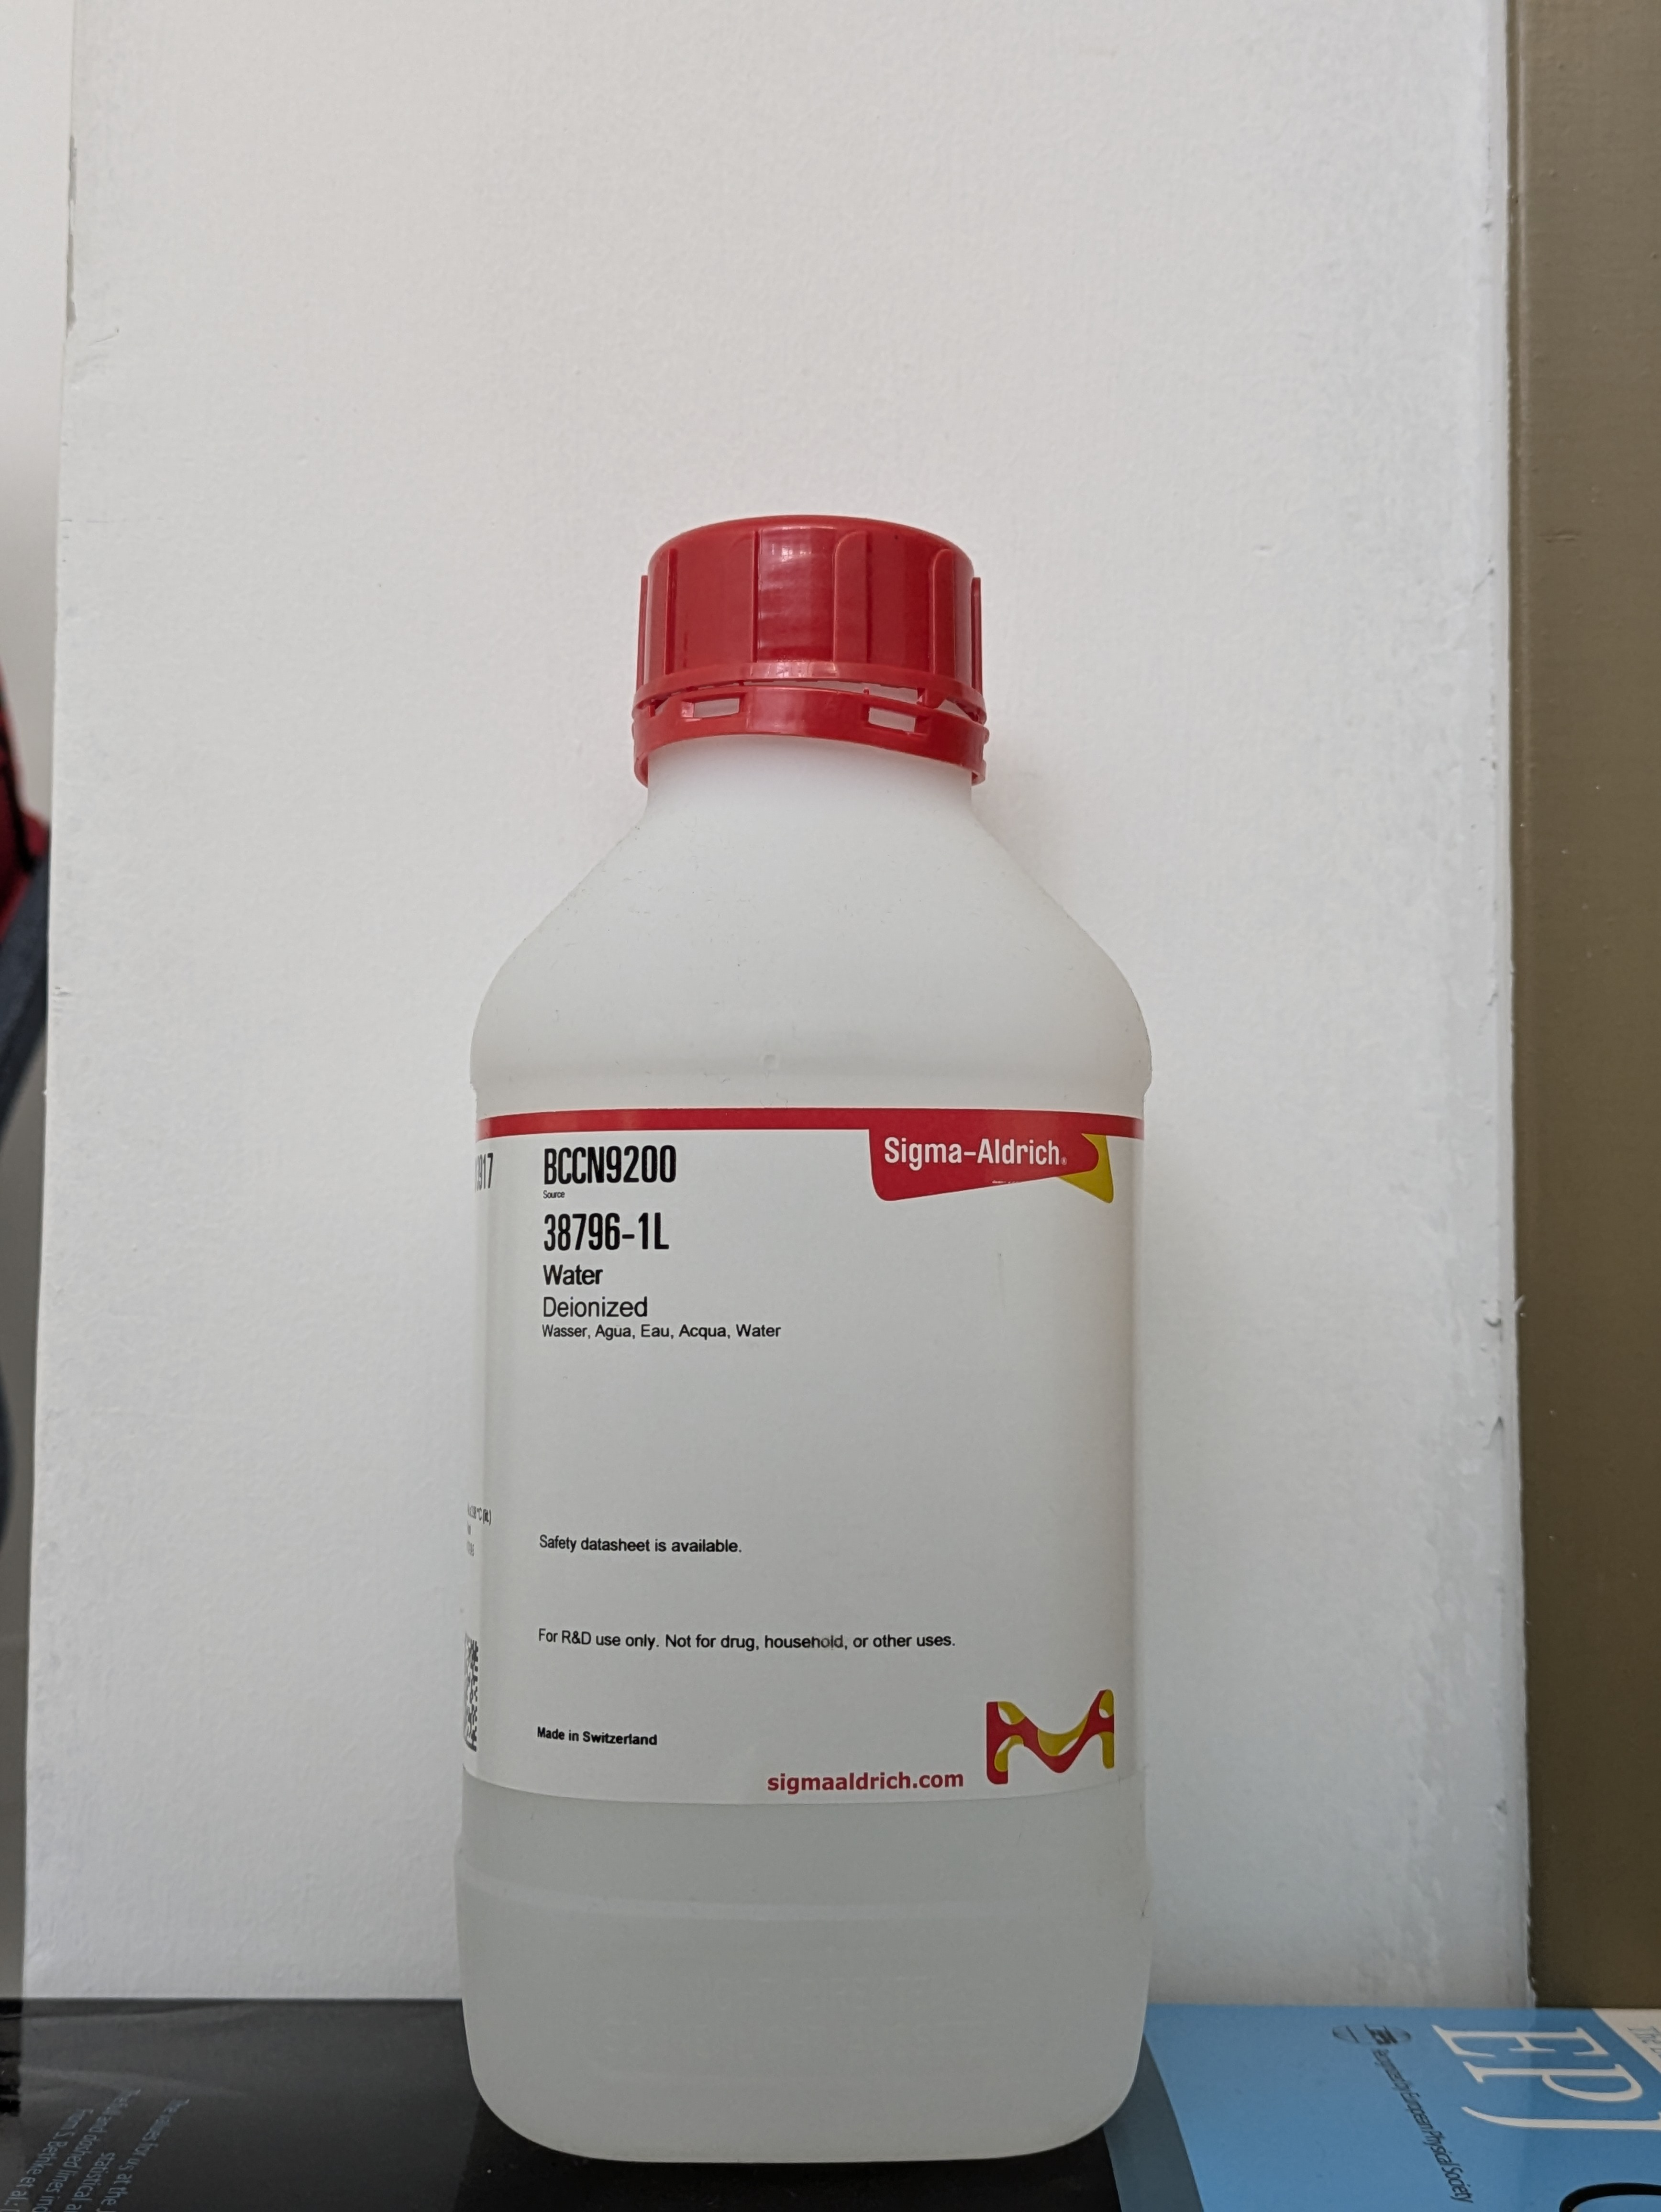
\includegraphics[width=\textwidth]{Images/DIW_lab.jpeg}
    \end{subfigure}
    \begin{subfigure}[b]{0.45\textwidth}
        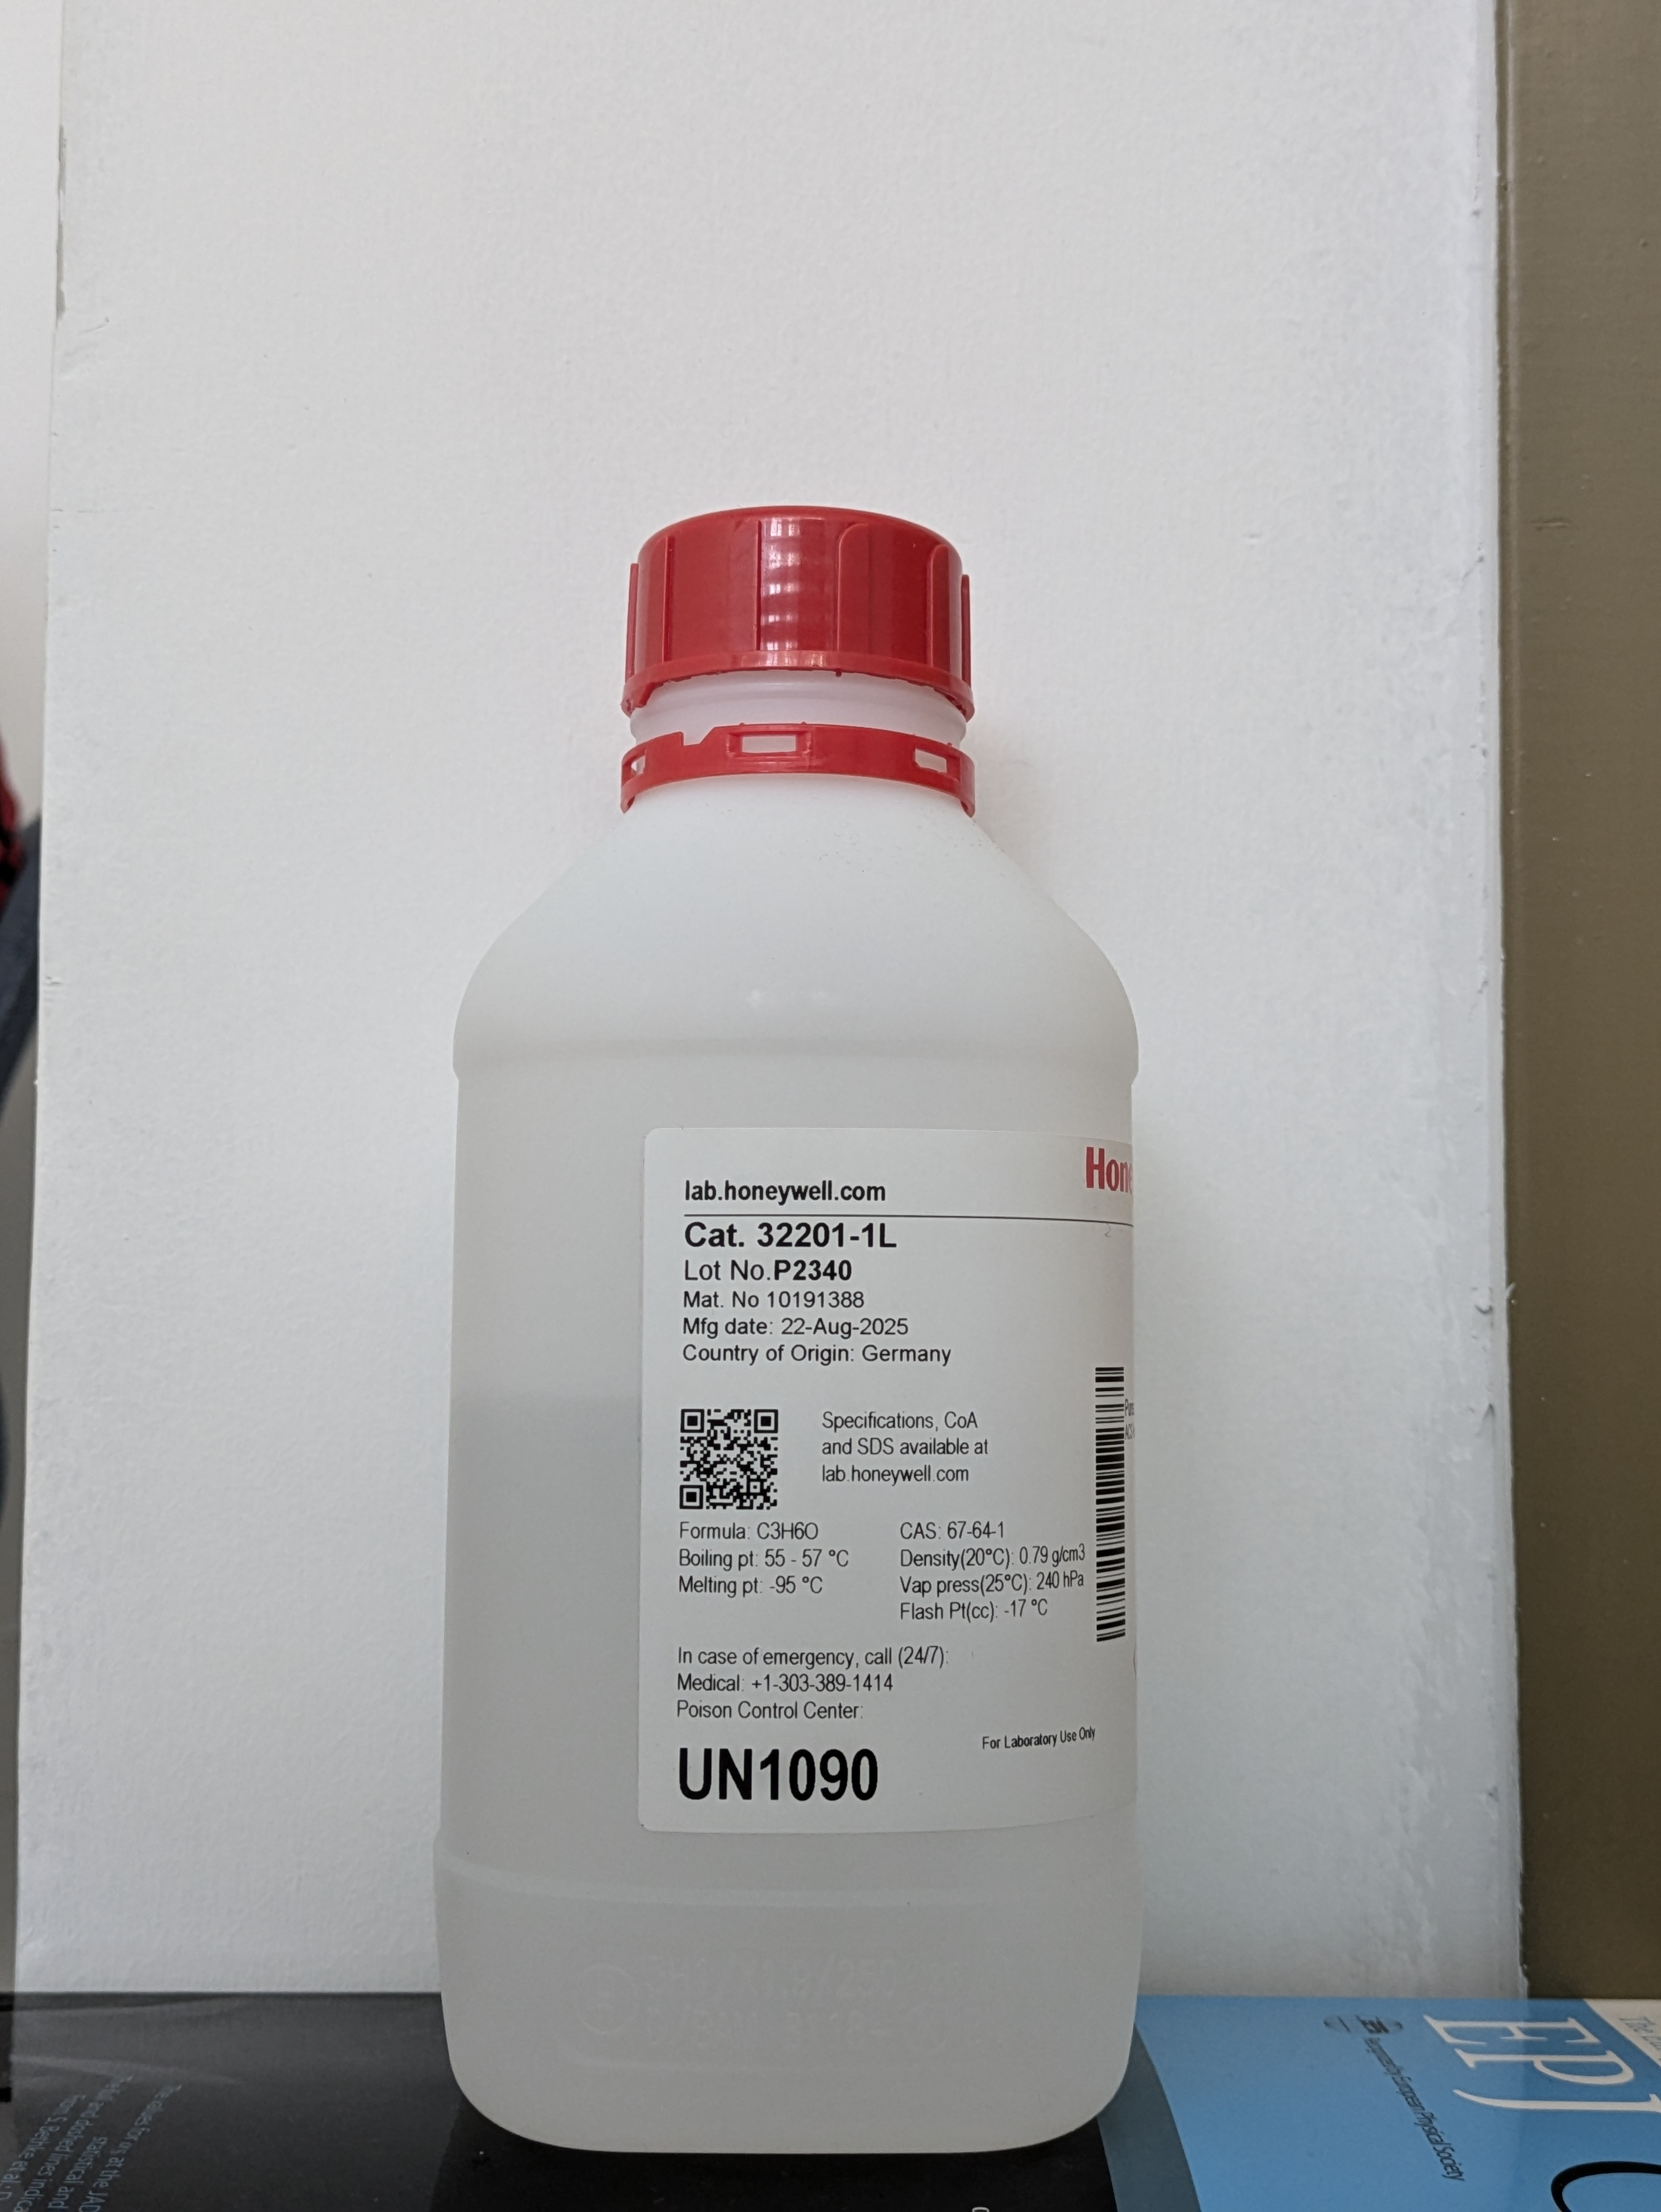
\includegraphics[width=\textwidth]{Images/acetone_lab.jpeg}
    \end{subfigure}
    \vfill
    \begin{subfigure}[b]{0.45\textwidth}
        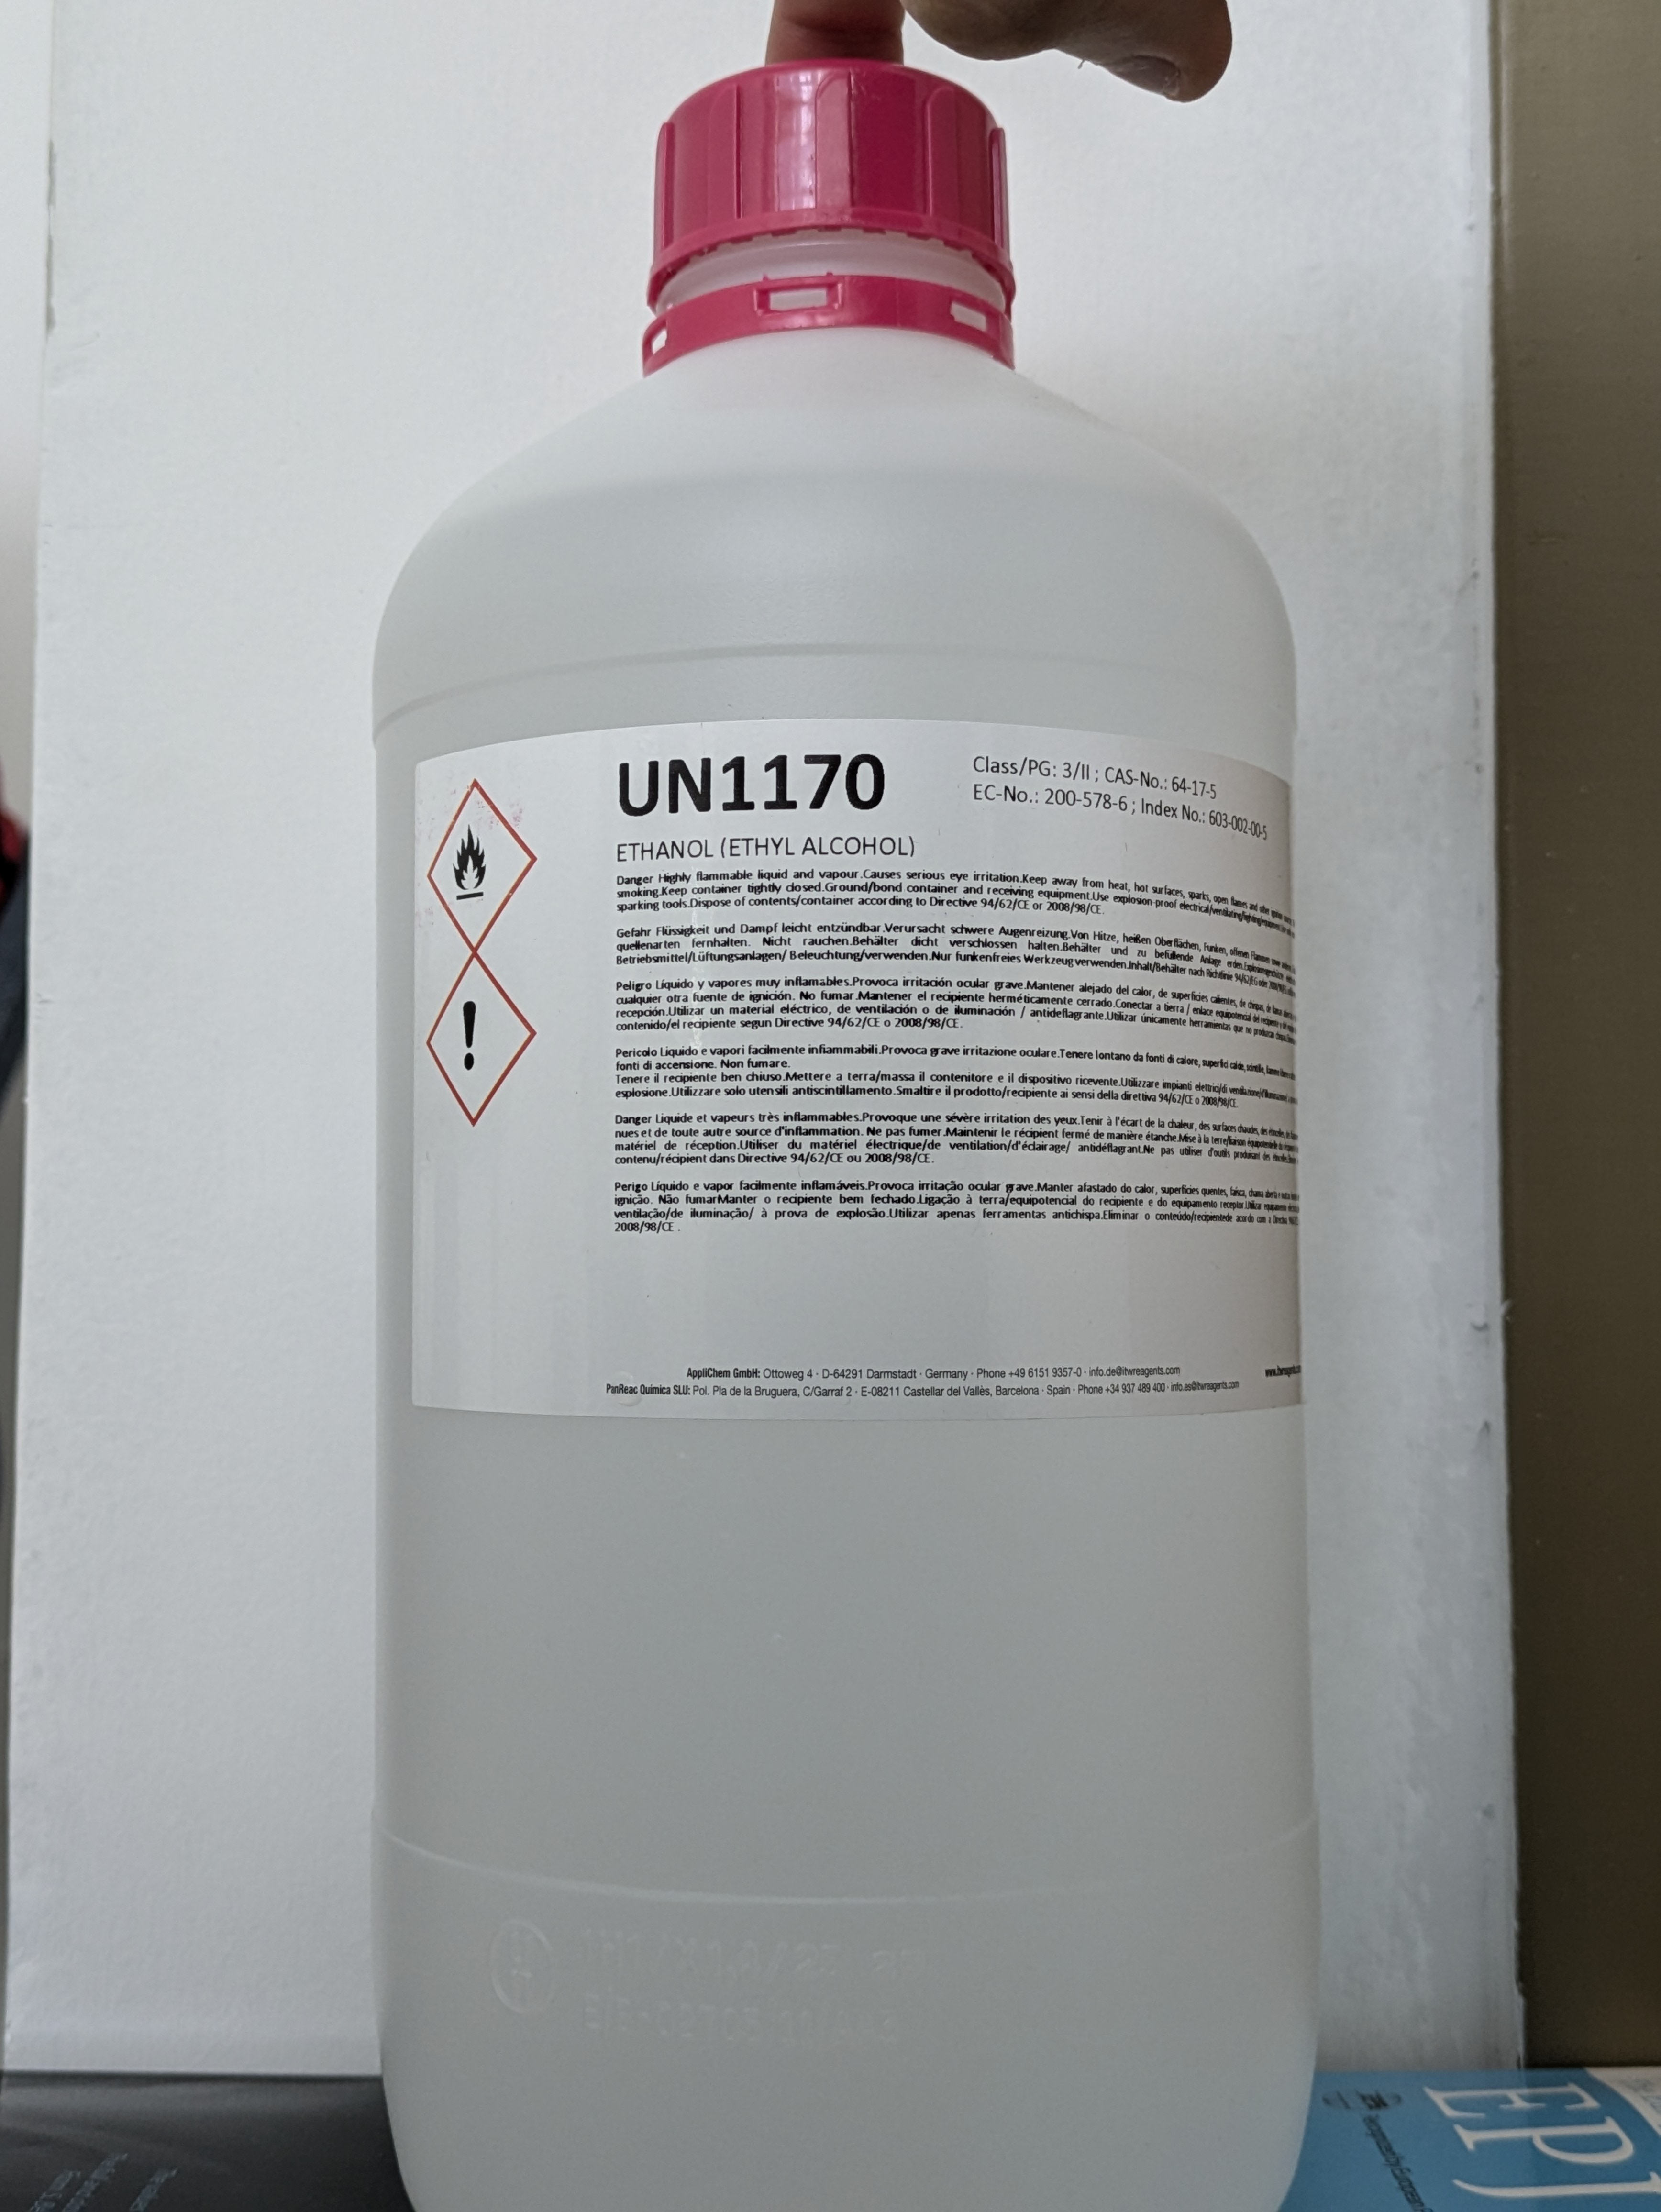
\includegraphics[width=\textwidth]{Images/ethanol_lab.jpeg}
    \end{subfigure}
    \begin{subfigure}[b]{0.45\textwidth}
        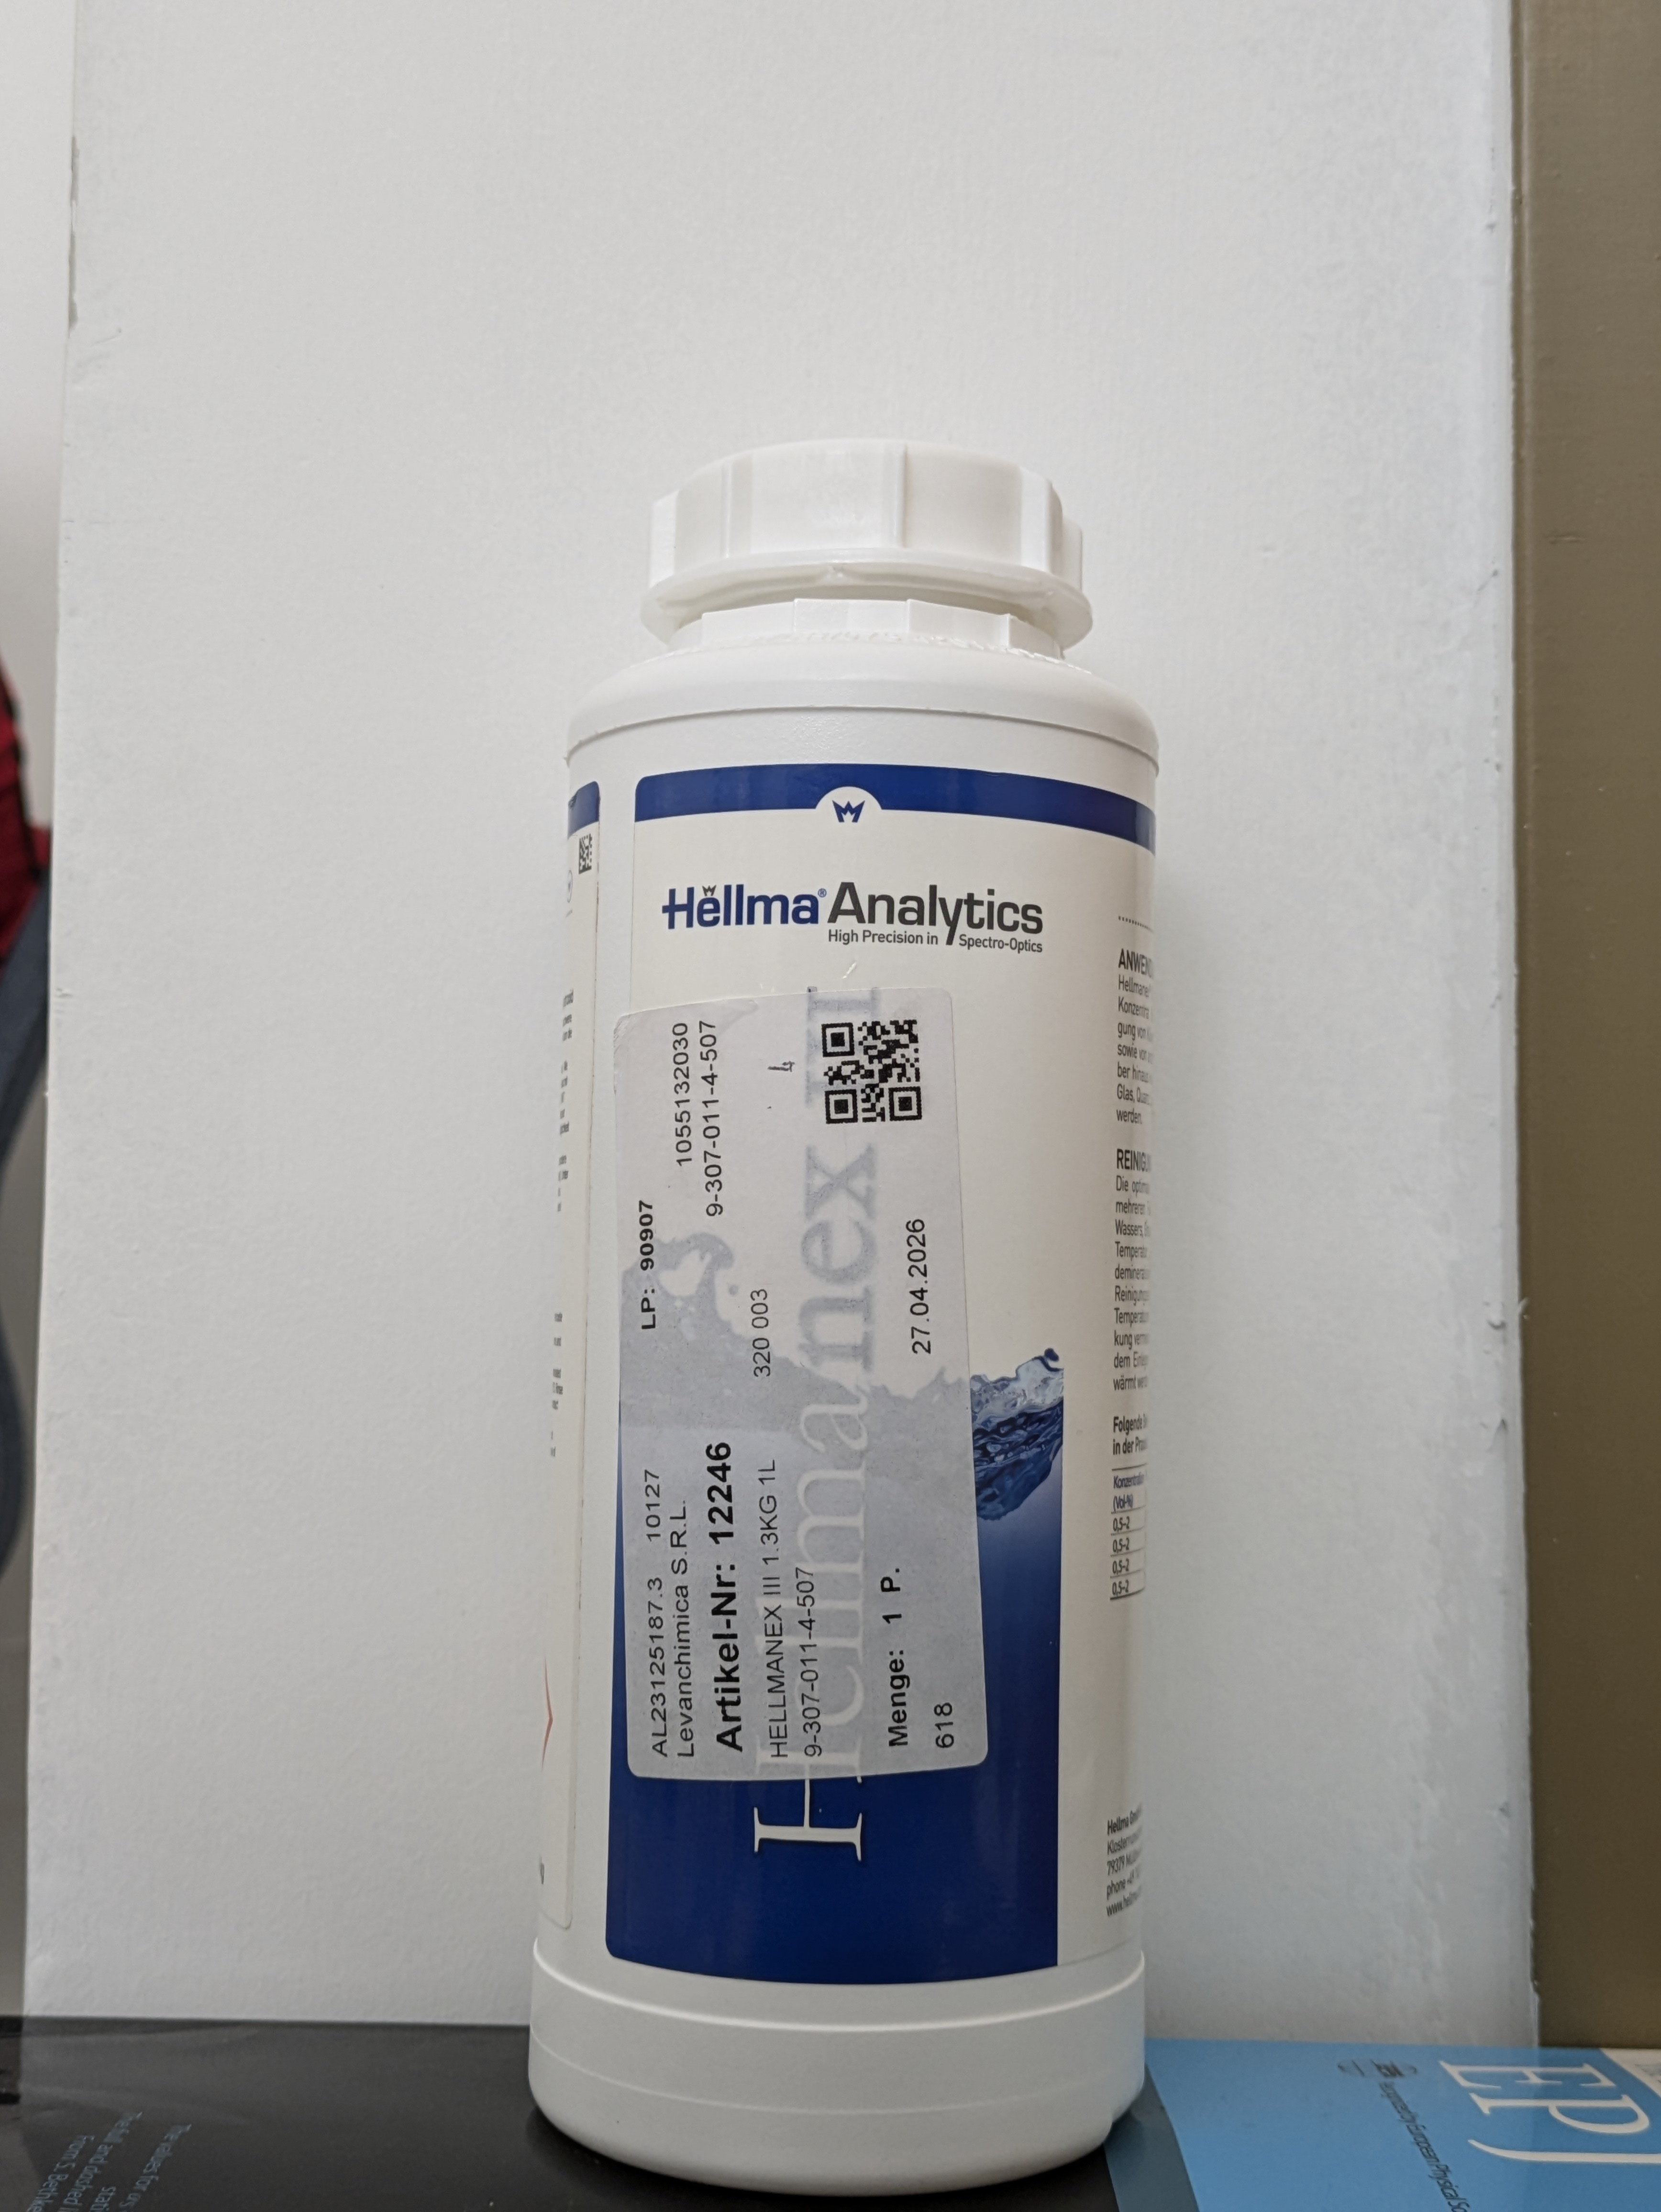
\includegraphics[width=\textwidth]{Images/soap_lab.jpeg}
    \end{subfigure}
    \caption{Chemicals employed in the experiment. 
    (1) Deionized Water (DIW) (2) Acetone (3) Ethanol (4) Hellmanex III soap}
    \label{fig:chemicals_lab}
\end{figure}